
\section*{Learning Objectives}

\begin{itemize}
\item Get you going on Algebra, just in case Calculus has erased it from your mind
\item Review on your own the quadratic equation.
\item Set the stage for cool things to come.
\end{itemize}

\section*{Outcomes}
\begin{itemize}
\item Refresher on the quadratic equation.
    \item Examples of systems of linear equations with two unknowns. Show that three things are possible when seeking a solution:
    \begin{itemize}
        \item there is one and only one solution (one says there is a unique solution, which is shorthand for ``there is a solution and it is unique'');
        \item there is no solution (at all); and
        \item there are an infinite number of solutions
    \end{itemize}

    \item Notation that will allow us to have as many unknowns as we'll need.
    \item Remarks that you can mostly ignore on why some numbers are called counting numbers, rational numbers, irrational numbers, or complex numbers
    \item Remarks on your first project.
    
    \item There is a programming manual associated with this book. Please see \url{https://www.dropbox.com/s/ev6v8veutdjhkuk/ROB_101_Julia_Programming_Guide.pdf?dl=0}.
    
\end{itemize}

\newpage

\section{For Review on Your Own: You Have Done Algebra Before}

\begin{tcolorbox}[sharp corners, colback=green!30, colframe=green!80!blue, title=\textbf{\large Quadratic Equation}]
$a x^2 + bx + c=0$, where $x$ is an \textit{unknown variable} and \textit{typically} $a$, $b$, and $c$ are fixed real numbers, called \textit{constants}. 

If $a \neq 0$, the solutions to this \textit{nonlinear algebraic equation} are 
$$x = \frac{-b \pm \sqrt{b^2-4ac}}{2a}, $$
where the symbol $\pm$ (read, plus minus) indicates that there is one solution $x$ corresponding to the plus sign and a second solution $x$ corresponding to the minus sign.\\

The \textit{discriminant} of a quadratic equation is $\Delta:=b^2-4ac.$
If $\Delta \ge 0$, the two solutions are \textit{real numbers}, while if  $\Delta <0 $, the two solutions are \textit{complex numbers}.
\end{tcolorbox}

\begin{tcolorbox}[title=\textbf{Complex Numbers}]
\textbf{If you have not learned complex numbers} (\textbf{a}lso \textbf{k}nown \textbf{a}s (\textbf{aka}) \textbf{\em imaginary numbers}) or are fuzzy on the details, let your GSI know. We may not use complex numbers at all in the graded portion of the course. We're not sure yet! We will need complex numbers when we study eigenvalues of matrices, which could happen at the end of the term, or it could be that we do not get that far. Piloting a Linear Algebra course during a pandemic has never been done before!
\end{tcolorbox}

\begin{example} 
\label{ex:QuadDistinctRealSolutions}
\textbf{(two distinct real solutions)} Find the roots of $2x^2 + 8x -10 =0$.


\end{example}

\textbf{Solution:}
\begin{align*}
        a=2, b&=8, c=-10\\
    b^2-4ac&= 144 >0\\
    x&=  \frac{-8 \pm \sqrt{144}}{4} \\
    &=  \frac{-8 \pm 12}{4} \\
    &= -2 \pm 3
    \end{align*}
    The two solutions are $x=1$ and $x=-5$.
\Qed

\begin{figure}[ht!]
\centering
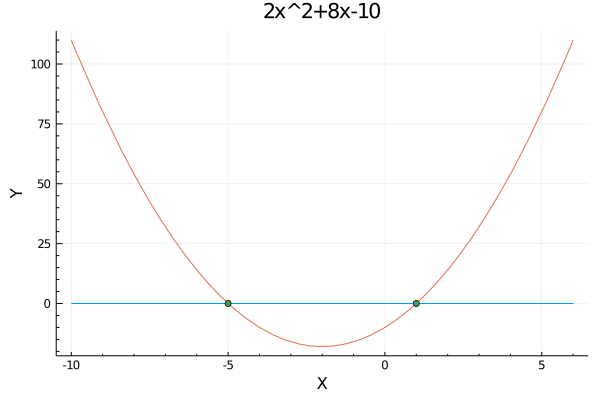
\includegraphics[width=0.5\textwidth]{Chap01_Intro/HandOut01_Fig01.png}
\caption[]{The two roots are at the intersection of the quadratic with the line $y=0$. Why? Because, by definition, the roots are values of $x$ where $ax^2 + bx + c$ equals zero!}
\end{figure}
    


% \noindent \textbf{Example two: two repeated real solutions}  $-x^2 - 4x -4 =0$
% \begin{align*}
%         a=-1, b&=-4, c=-4\\
%     b^2-4ac&= 0\\
%     x&=  \frac{4 \pm \sqrt{0}}{-2} \\
%     &=  \frac{4 \pm 0}{-2} \\
%     &= -2 \pm 0
%     \end{align*}
%     The two solutions are $x=-2$ and $x=-2$.
\newpage
\begin{example}
\label{ex:QuadRepeatedRealSolutions}
\textbf{(two repeated real solutions)}  Find the roots of $2x^2 +8 x + 8 =0$.
\end{example}

\textbf{Solution:}
\begin{align*}
        a=2, b&=8, c=8\\
    b^2-4ac&= 0\\
    x&=  \frac{-8 \pm \sqrt{0}}{4} \\
    &=  \frac{-8\pm 0}{4} \\
    &= -2 \pm 0
    \end{align*}
    The two solutions are $x=-2$ and $x=-2$.
\Qed
 

\begin{figure}[hbt!]
\centering
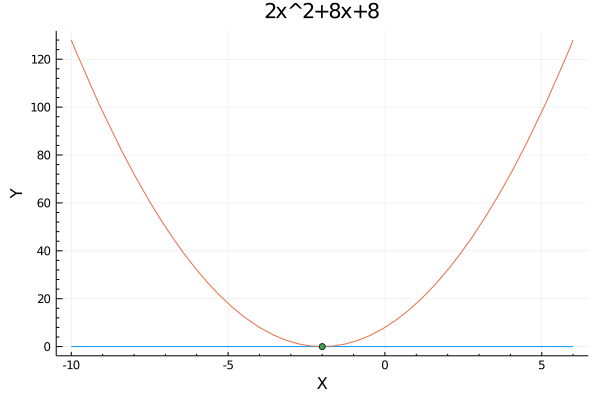
\includegraphics[width=0.5\textwidth]{Chap01_Intro/HandOut01_Fig02.png}
\caption[]{Note that there is now only a single intersection with $y=0$ at $x=-2$. Because quadratic equations have two solutions, we say \textbf{the root at $\mathbf{x=-2}$ is repeated}.}
\end{figure}




\begin{example}
\label{ex:QuadDistinctComplexSolutions}
\textbf{(two distinct complex solutions)}  Find the roots of $2x^2 +8 x + 10 =0$.
\end{example}

\textbf{Solution:}

\begin{align*}
        a=2, b&=8, c=10\\
    b^2-4ac&= -16\\
    x&=  \frac{-8 \pm \sqrt{-16}}{4} \\
    &=  \frac{-8\pm\sqrt{16} \sqrt{-1}}{4} \\
      &=  \frac{-8\pm 4\sqrt{-1}}{4} \\
       &=  -2\pm \sqrt{-1} \\
    &= -2 \pm i
    \end{align*}
    The two solutions are $x=-2+i$ and $x=-2-i$, where $i:=\sqrt{-1}$ is an \textit{imaginary number}. If you have not already learned complex numbers, do not sweat it. If we need them at all in ROB 101, it will be at the end of the term and we will teach complex numbers before we use them!
\Qed

    
\begin{figure}[hbt!]
\centering
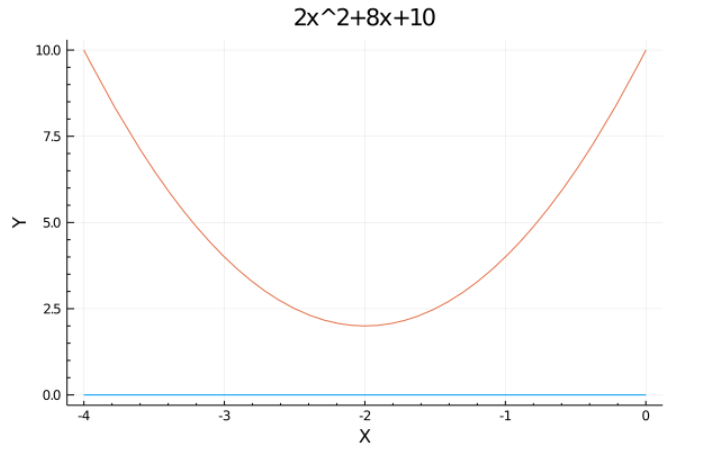
\includegraphics[width=0.5\textwidth]{Chap01_Intro/HandOut01_Fig03.png}
\caption[]{Note that there are no intersections with $y=0$ and hence there are not any real solutions.}
\end{figure}


\newpage

\noindent \textbf{Remark:} As in many subjects, the vocabulary in mathematics reflects the many twists and turns of history. If you are expecting mathematics to be a \textit{pure science} in the sense that it is 100\% logical, then you will often be disappointed! The Greeks and Egyptians called $1, 2, 3, \ldots$ \textit{natural numbers} or \textit{counting numbers} because they arose ``naturally'' in ``counting objects'': one cow, two sheep, three coins, four sacks of flour, etc. They were also comfortable with \textit{fractions},  $\frac{m}{n}$, where both $m$ and $n$ were counting numbers, and hence, $n$ could never be zero. Fractions were called \textit{rational numbers} based on the word \textit{ratio}.
The square root of two, $\sqrt{2}$, was known to the Babylonians, Indians and Greeks.
Our notion of $\sqrt{2}$ is probably thanks to Pythagoras, the Ionian Greek philosopher known to you for developing the Pythagorean Theorem relating the sides of right triangles, yes, the famous formula $a^2+b^2=c^2$, which gives $1^2 + 1^2 = (\sqrt{2})^2$, where the symbol $\sqrt{2}$ stands for the ``quantity that when squared gives the counting number $2$''. It took a long time for the Greeks to accept that $\sqrt{2}$ could not be written as a \textit{ratio of two counting numbers}. Eventually, it was proved to be \textit{irrational}, that is, \textit{not rational}, which means precisely that it cannot be expressed as the ratio of two counting numbers. In case you are interested, while Euclid was not the first to prove $\sqrt{2}$ was irrational, the beautiful reasoning he invented for the proof of $\sqrt{2}$ not being a rational number is still taught today. It is called \textit{proof by contradiction}\footnote{It may seem remarkable to you that the two words ``proof'' and ``contradiction'' can coexist in logical statements. As you advance in your mathematical training, you may come across the term again. ``Proof by contradcition'' is not for amateurs...think about it as semi-professional-grade logic and math.}. \\

So far, so good with regards to vocabulary. But why call things involving $\sqrt{-1}$ complex numbers? Initially, mathematicians could not justify the existence of \textit{quantities involving square roots of negative numbers.} Using them in calculations was a sign of ``careless'' mathematics and such numbers were treated as being \textit{figments of one's imagination}, literally, \textit{imaginary numbers}. Nevertheless, some (brave) mathematicians found them convenient for solving equations and others even for describing physical phenomena. Eventually, formal algebra caught up with the notion of imaginary numbers and their rules of use were rigorously justified. The name imaginary numbers stuck, however! Here is a link to a slightly simplified explanation of how mathematicians ``codify'' the existence of complex numbers:  \url{http://www.math.toronto.edu/mathnet/answers/imagexist.html} Your instructors are unsure if they could have followed the reasoning in this document when they were at your stage of college, so do not sweat it.\\

Just for fun, you might want to learn more about numbers on Wikipedia \url{https://en.wikipedia.org/wiki/Number}. Were negative numbers always accepted? What about the notion of zero? \textbf{None of these remarks on numbers are required reading}. You will not be tested on the history of numbers!\\

\begin{tcolorbox}[title=\textbf{To Know}]
\begin{itemize}
    \item What are the counting numbers (also known as the natural numbers)? 
    \item What are rational numbers?
    \item Be able to give an example of an irrational number, but of course, you are not expected to prove it is irrational. 
    \item Later in the course (though it is not sure): what are imaginary numbers? 
\end{itemize}
\end{tcolorbox}

\newpage

\noindent \textbf{In ROB 101}, the first ten Chapters focus on linear equations, hence, equations that do not have quadratic terms $x^2$, cubic terms $x^3$, nor terms with higher powers; they also do not have $\sin(x)$, $\cos(x)$, $\sqrt{x}$, or $e^x$ or anything like that. It is perhaps hard to believe that equations with only order-one terms and constants could be interesting or important, but they are both interesting and important! 

\section{Linear Systems of Equations: What can happen?}
\label{sec:WhatCanHappen}

We begin with several examples to illustrate what can happen.\\

\noindent \textbf{Same number of equations as unknowns, and there is a unique solution:}
\begin{equation}
\label{eq:SLE:Ex1}
\begin{aligned}
x+y &=4 \\
2x-y&=-1
\end{aligned}
\end{equation}
One way to compute a solution is to solve for $x$ in terms of $y$ in the first equation and then substitute that into the second equation,
\begin{align*}
x+y =4 & \implies x = 4-y\\
2x-y=-1 & \implies 2(4-y)-y=-1\\
& \implies -3y=-9 \\
& \implies y = 3\\
&\text{going back to the top}\\
x = 4-y & \implies x=1
\end{align*}
You can try on your own solving for $y$ in terms of $x$ and repeating the above steps. You will obtain the same answer, namely $x=1, y=3$. 

Another ``trick'' you can try, just to see if we can generate a different answer, is to add the first equation to the second, which will eliminate $y$,
\begin{align*}
x+y &=4 \\
+~ 2x-y&=-1\\ \vspace*{-0.2cm}
\mathclap{\rule{2cm}{0.4pt}}& \mathclap{\rule{1.5cm}{0.4pt}} \vspace*{-0.2cm} \\
 3x + 0 y & =3 \\
 & \implies x=1 \\
\end{align*}
Going back to the top and using either of the two equations
\begin{align*}
 x+y =4 & \implies y = 4-x \\
 & \implies y = 3 \\
& \text{or} \\
 2x-y=-1 &\implies -y = -2x - 1\\
 & \implies -y = -3\\
 & \implies y = 3
\end{align*}
gives the same answer as before, namely,  $x=1, y=3$. \\

In fact, the set of equations \eqref{eq:SLE:Ex1} has one, and only one, solution. In math-speak, one says the set of equations \eqref{eq:SLE:Ex1} has a \textit{unique solution}. Often, we will stack $x$ and $y$ together and write the solution as
$$\begin{bmatrix} x \\ y\end{bmatrix} = \left[\begin{array}{l}
1 \\ 3 \end{array}  \right].$$

\noindent \textbf{Same number of equations as unknowns, and there is no solution:}
\begin{equation}
\label{eq:SLE:Ex2}
\begin{aligned}
x-y &=1 \\
2x-2y&=-1
\end{aligned}
\end{equation}
Because there are only two equations with a very nice set of numbers you might notice almost immediately that the left-hand side of the second equation is twice the left-hand side of the first equation, namely, $2 x - 2y = 2(x-y),$ but when we look to the right-hand sides, $-1 \neq 2 \cdot 1$, and hence the equations \eqref{eq:SLE:Ex2} are \textit{inconsistent}. \\

While the above is one way to analyze the problem, let's try to find a solution just as we did for the first set of equations, 
\begin{align*}
x-y =1 & \implies x = y+1 \\
2x-2y=-1&  \implies 2(y+1)-2y = -1\\
& \implies 2 + 2y - 2y = -1 \\
& \implies 2 = -1.
\end{align*}
Hence, trying to solve the equations has led us to a \textit{contradiction}, namely $2=-1$. Perhaps if we had solved for $y$ in terms of $x$, we could have found a solution? Let's try
\begin{align*}
x-y =1 & \implies -y = -x+1 \\
& \implies y = x-1 \\
2x-2y=-1&  \implies 2x-2(x-1) = -1\\
& \implies 2x -2x +2 = -1 \\
& \implies 2 = -1
\end{align*}
again! No matter how you manipulate the equations \eqref{eq:SLE:Ex2}, while obeying ``the rules of algebra'' (which we have \textbf{not yet learned} for systems of linear equations), you cannot extract a sensible answer from these equations. They really are \textit{inconsistent}. \\

\noindent \textbf{Same number of equations as unknowns, and there are an infinite number of solutions:}
\begin{equation}
\label{eq:SLE:Ex3}
\begin{aligned}
x-y &=1 \\
2x-2y&=2
\end{aligned}
\end{equation}
Because there are only two equations with a very nice set of numbers, you might notice that the left-hand side of the second equation is twice the left-hand side of the first equation, namely, $2 x - 2y = 2(x-y),$ and this time, when we look to the right-hand sides, $2= 2 \cdot 1$, and hence the two equations are actually the ``same'' in the sense that one equation can be obtained from the other equation by multiplying both sides of it by a non-zero constant. We could elaborate a bit, but it's not worth it at this point. Instead, let's approach the solution just as we did in the first case.\\

We solve for $x$ in terms of $y$ in the first equation and then substitute that into the second equation,
\begin{align*}
x-y =1 & \implies x = y+1\\
2x-2y=2 & \implies 2(y+1)-2y=2\\
& \implies 2y + 2 - 2y =2 \\
& \implies 2 = 2.
\end{align*}
The conclusion $2=2$, is perfectly correct, but tells us nothing about $y$. In fact, we can view the value of $y$ as an arbitrary \textit{free parameter} and hence the solution to \eqref{eq:SLE:Ex3} is 
$$x=y+1,~~ -\infty < y < \infty.$$
The solution can also be expressed as
$$ y = x-1,~~ -\infty < x < \infty,$$
which perhaps inspires you to plot the solution as a line in $\real^2$, with slope $m=1$ and $y$-intercept $b=-1$.\\



\begin{tcolorbox}[sharp corners, colback=green!30, colframe=green!80!blue, title=\textbf{\large Summary So Far}]
Consider a set of two equations with two unknowns $x$ and $y$
\begin{equation}
\label{eq:SLE:Ex4}
\begin{aligned}
a_{11}x + a_{12}y &=b_1 \\
a_{21}x + a_{22}y&=b_2,
\end{aligned}
\end{equation}
constants $a_{11}, a_{12}, a_{21}, a_{22}$ and $b_1, b_2$. Depending on the values of the constants, the linear equations \eqref{eq:SLE:Ex4} can have a unique solution, no solution, or an infinity of solutions. The equations cannot have two and only two distinct solutions. 
\end{tcolorbox}

\noindent \textbf{More equations than unknowns typically means that there are no solutions:}
The system of equations
\begin{equation}
\label{eq:SLE:Ex6}
\begin{aligned}
x&=1 \\
y&=2 \\
x+y&=a
\end{aligned}
\end{equation}
will only have a solution when $a=3$. For all other values of $a$, it will not have a solution. We will learn to recognize later when the set of equations are consistent. At this point in the course, we do not have adequate mathematical tools to address the issue.

\vspace*{1cm} 

\begin{tcolorbox}[title=\textbf{\Large Limit of Hand Solutions}]
When there are only two equations and two unknowns, determining \textit{by hand} if the equations have one solution, no solution, or an infinity of solutions is quite do-able. With sufficient motivation and ``nice numbers'', three equations and three unknowns is also not too bad. At four, it becomes super tedious and errors begin to sprout like weeds. Hence, what about 100 equations and 100 unknowns? \textbf{Our four-week goal is for you to handle systems of linear equations with hundreds of variables with confidence and ease} As you can imagine, this is where the ``computational'' part of ROB 101's name comes into play!
\end{tcolorbox}

\section{Naming Variables}

If we have two variables (also called unknowns), it is natural to call them $x$ and $y$. If we have three variables, naming them $x$, $y$, and $z$ works fine. If we have $26$ variables, would we start with $a$ and go all the way to $z$? What if we have more variables? Well, there are $24$ Greek letters, do we add them to the list? Throw in Mandarin Characters to get us to several thousand variables? Clearly, this is not a practical way to go. The only real possibility is to add counting numbers, because there are as many of them as we need, and computers understand numbers!\\

\textbf{Welcome to $x_1, x_2, x_3, \ldots, x_n$, or $y_1, y_2, \ldots, y_m$ etc.}

\section{A 3 x 3 Example}
Here is a \textit{system of linear equations} with variables $x_1, x_2, x_3$. 
\begin{equation}
\label{eq:SLE:Ex5}
\begin{aligned}
x_1+x_2+2x_3 &=7 \\
2x_1-x_2+x_3&=0.5\\
x_1 + 4 x_3 &=7
\end{aligned}
\end{equation}
The strategy for seeking a solution is the same as with two equations and two unknowns: solve for one of the variables in terms of the other variables, substitute into the remaining equations, simplify them, and repeat. We can start anywhere, so let's solve for $x_1$ in the bottom equation and plug that back into the two equations above it. Doing so gives us,
\begin{equation}
\label{eq:SLE:Ex5b}
   x_1 = 7 - 4 x_3 
\end{equation}
and then 
\begin{align*}
\underbrace{( 7 - 4x_3)}_{x_1} +x_2+ 2x_3 =7 & \implies x_2  - 2 x_3 = 0 \\
\underbrace{2( 7 - 4x_3)}_{2 x_1}-x_2+x_3=0.5 & \implies -x_2 -7 x_3 = -13.5
\end{align*}
\begin{align}
\label{eq:SLE:Ex5c}
 x_2  - 2 x_3 = 0 &\implies x_2 = 2 x_3\\
 -x_2 -7 x_3 = -13.5 & \implies \underbrace{-(2 x_3)}_{-x_2}-7x_3 = -13.5 \nonumber \\
 & \implies - 9 x_3 = -13.5  \nonumber\\
 &\implies x_3 = 1.5 \nonumber
\end{align}
Plugging ``$x_3=1.5$'' into \eqref{eq:SLE:Ex5b} gives $$x_1=7-4\cdot (1.5)=7-6=1.$$ 
And then from \eqref{eq:SLE:Ex5b}, we have that
$$x_2 = 2 x_3 = 2 \cdot (1.5) = 3. $$
Hence, the solution is
\begin{equation}
    \begin{bmatrix} x_1 \\ x_2 \\ x_3 \end{bmatrix} = \left[\begin{array}{l}
1.0 \\ 3.0 \\ 1.5
\end{array}  \right].
\end{equation}

% \section{Square Systems of Linear Equations: $n$ equations and $n$ unknowns}

% Finally, we'll write down a system of $n\ge 1$ linear equations with $n\ge1$ unknowns (or variables) $x_1, x_2, \ldots, x_n$. 

% \begin{equation}
% \label{eq:nbynSystemLinearEquations}
%     \begin{array}{cccc}
%          &  \\
%          & 
%     \end{array}
% \end{equation}
\vspace*{.5cm}
\begin{tcolorbox}[sharp corners, colback=green!30, colframe=green!80!blue, title=\textbf{\Large Tedium and Pain $\boldsymbol{\implies}$ Motivation!}]
The hope is that you found the $3 \times 3$ example super tedious and something you'd prefer to avoid! The more tedious and painful you found it, the more motivation you will have to learn some new math that will make solving systems of linear equations a snap.
\end{tcolorbox}

\section{Greek Alphabet}
It's hard to believe that the 26 Latin letters we know and love, $a, b, c, \ldots, x, y, z$, especially after being augmented with numerical subscripts, do not provide enough symbols! You might as well get used to it, \textbf{engineers and mathematicians often use the 24 Greek letters as well:} $\alpha, \beta, \gamma, \ldots, \chi, \psi, \omega$. 
Here is a link to the Greek alphabet with names of the letters and their pronunciations: \url{https://web.mit.edu/jmorzins/www/greek-alphabet.html}.  99.9\% of all engineers, including your author, mispronounce them, so do not feel intimidated by that. Just gleefully join the club! \\

There are several accepted modern pronunciations of the Greek alphabet, it seems, giving you even less worry about your own pronunciation. The links below give a few of them:  
\begin{enumerate}
 \item Greek Alphabet - Pronunciation of each letter: \url{https://www.youtube.com/watch?v=1FyEWbwBarQ}
 
    \item Greek Alphabet Rap Song: \url{https://www.youtube.com/watch?v=w3D5ERMOpMk} 

 \item Greek Alphabet Song (Nursery-rhyme Style):  \url{https://www.youtube.com/watch?v=3gaeIUsPJ-Y}
 
 
 \item Learn the Greek Alphabet in Less Than 10 Minutes:  \url{https://www.youtube.com/watch?v=BQVoz-HX2cA}

 \end{enumerate}
 If you lookup the origin of the word ``AlphaBet'', you will learn that it comes from Alpha Beta, the first two letters of the Greek Alphabet. 


\section{(Optional Read) Where is Computational Linear Algebra Used? }


Figure~\ref{fig:ApplicationsLinearAlgebra} shows numerous areas where Computational Linear Algebra is used. In ROB 101, we have built projects around three different themes to give you a chance to really dive into a subject and feel that you learned something beyond the math itself:
\begin{itemize}
    \item For \textbf{Project 1: Map Building from LiDAR Data} you will be given data collected on the Cassie Blue bipedal robot during an experiment on the North Campus Grove and are asked to transform the data for building a map and visualizing it using Julia. The underlying work you will do is very similar to what is done in real-time\footnote{Real-time means the computations are done quickly enough on the robot that they can be used almost immediately. This is opposed to ``off-line'' where you collect data on the robot and then do the processing on a desktop in the lab. You are clearly doing offline data processing, which is easier, because there are no computation time requirements.} on Cassie in order to build a map for autonomous navigation. You may wish to view the videos \url{https://www.youtube.com/watch?v=pNyXsZ5zVZk} and \url{https://youtu.be/gE3Y-2Q3gco} to see mapping and navigation done in real-time. Yes, this is very similar to what is done by AVs (Autonomous Vehicles). One difference is that an AV has 200 Kg of electronics in its trunk to process all the data, while Cassie's entire autonomy package weighs in at 9 Kg and runs off a hobbyist LiPo battery. 
    \item For \textbf{Project 2: Precipitation Data in Alaska (A True Story)}, you will use linear regression methods taught in Chap.~\ref{chap:NormRegression} and apply them to a much larger dataset from the U.S. National Oceanic and Atmospheric Administration (NOAA). The project will give you insight into Machine Learning, one facet of the burgeoning area of Artificial Intelligence or AI for short. You will learn an important new function called the radial basis function and apply it towards building a mathematical model of a surface.
    \item For \textbf{Project 3: Feedback Control of a Segway}, you will learn how to balance and ``drive'' an inherently unstable mobile robot! If you have not seen a Segway, here is a video of the bideal robot Cassie Blue riding a Segway \url{https://youtu.be/0gauVSUJzd0}. Your project will not be this awesome, but the project will put you on the road to awesome things!
\end{itemize}

Now, in case just reading about these projects intimidates you, we want to assure you that their difficulty has been thoughtfully scaled to a first-semester Y1 experience, while also giving you insight into how the real things are done. This is possible because we will teach you math and programming in an integrated manner. The math reinforces the programming and the programming reinforces the math. At each step of the way, you will increase your confidence in Engineering, Mathematics, or the Sciences as a career choice. In High School, you were mostly taught math as being disconnected from real applications. There was a huge emphasis on memorizing formulas or theorems, without ever really using the concepts to do something fun. In ROB 101, we hope to show you how empowering it is to do mathematics at the scale of life.

\section{Looking Ahead}

We need a straightforward way to check whether a set of equations falls into the nice case of having a unique solution or is it one of the ``problematic cases'' where there may be no solution at all or an infinity of solutions. 
To get there, we need to learn:
\begin{itemize}
\item what are \textit{matrices} and \textit{vectors};
    \item how to express a system of linear equations in terms of \textit{matrices} and \textit{vectors};
    \item what it means for a set of linear equations to be \textit{triangular} or \textit{square}; and
    \item what is the \textit{determinant} of a matrix. 
\end{itemize}


%\clearpage

 
     \begin{figure}[hbt!]
\centering
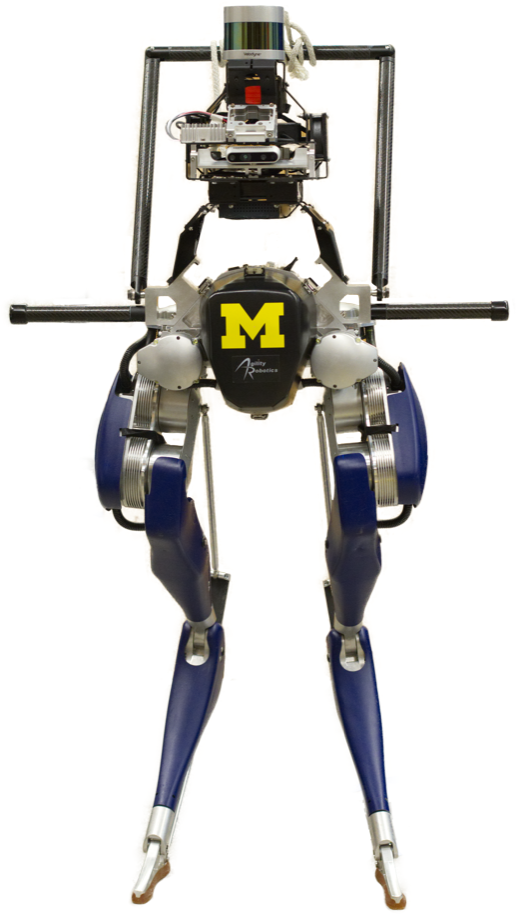
\includegraphics[width=0.2\textwidth]{Chap01_Intro/CassieTorso_ClearBackground_TightBorder.png}
\caption{Cassie Blue with her perception package: a 32-Beam Velodyne LiDAR and an Intel RealSense Camera. In your first project, you will learn what is a LiDAR sensor and how to process the LiDAR data to build a ``map'' that a robot can use for navigation. Each colored dot in Fig.~\ref{fig:LiDARmap} is a LiDAR measurement. How many are there? Ten thousand, maybe? The image is the result of combining multiple LiDAR scans into a single image. You will learn that this involves applying matrices to vectors. You will learn about coordinate frames. Right now, this seems like magic. In a few weeks, you will be comfortable enough with the Julia programming language to manipulate a dataset with 10,000 points or more. \textbf{Remember, one of our goals is mathematics and programming at the scale of life!} }
\end{figure}




\begin{figure}[b!]%
\centering
\subfloat[]{%
    \label{fig:LiDARmap}%
	\centering
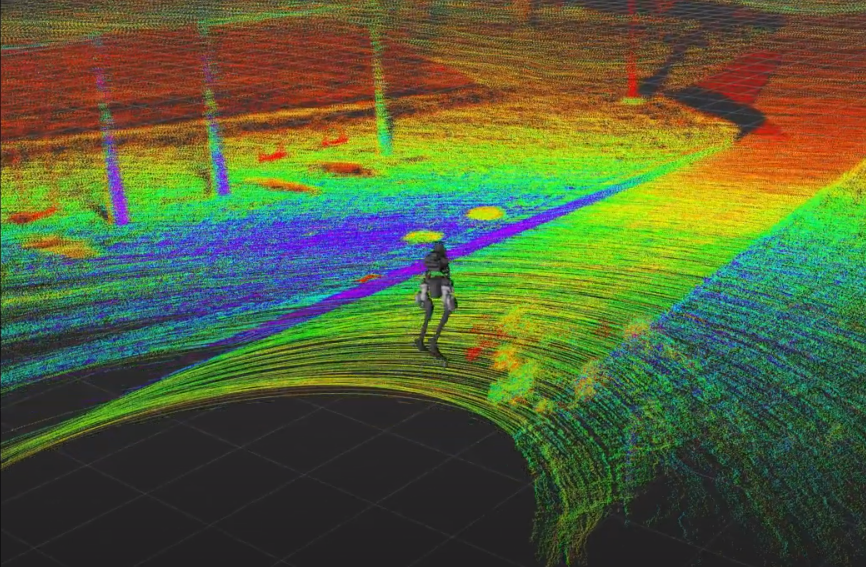
\includegraphics[width=0.45\columnwidth]{Chap01_Intro/RegisteredLiDARscans.png}}%
\hspace{5pt}%
\subfloat[]{%
    \label{fig:Regression}%
	\centering
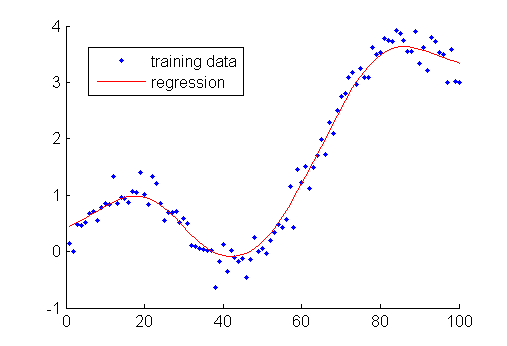
\includegraphics[width=0.42\columnwidth]{Chap01_Intro/Gaussian_Kernel_Regression.png}}%
\hspace{5pt}%
\subfloat[]{%
    \label{fig:Segway}%
	\centering
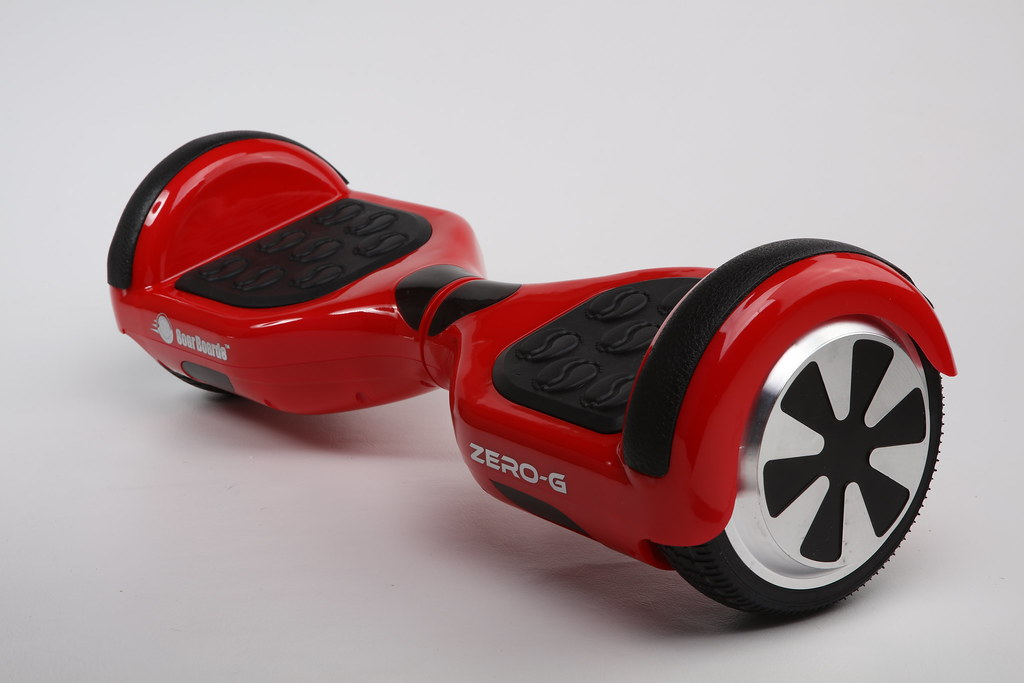
\includegraphics[width=0.47\columnwidth]{Chap01_Intro/Segway.jpg}}%
\hspace{5pt}%
    \subfloat[]{%
    \label{fig:GradientDescentIntro}%
	\centering
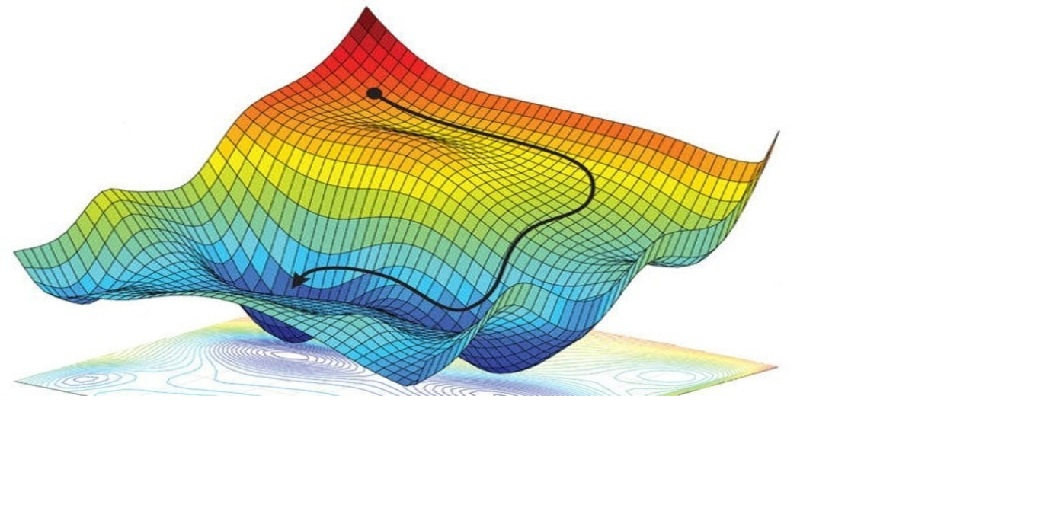
\includegraphics[width=0.4\columnwidth]{Chap01_Intro/GradientDescent02.jpg}}%
\hspace{5pt}%
\subfloat[]{%
    \label{fig:CameraCalibration}%
	\centering
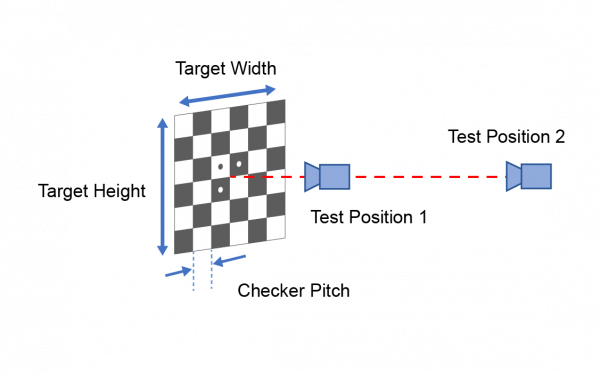
\includegraphics[width=0.48\columnwidth]{Chap01_Intro/cameraCalibration.png}}%
\hspace{5pt}%
\subfloat[]{%
    \label{fig:ResistorOpAmp}%
	\centering
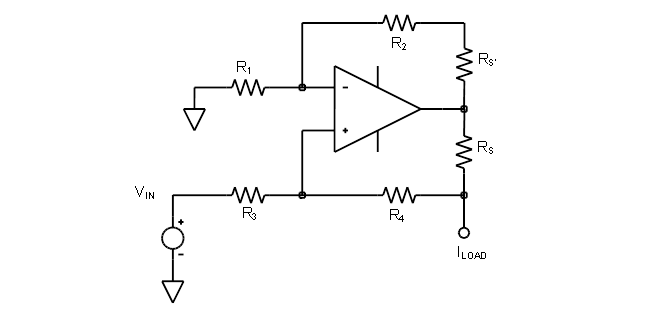
\includegraphics[width=0.5\columnwidth]{Chap01_Intro/ResistorOpAmp.png}}%
    \caption[]{Just a few of the almost infinitely many application areas  of linear algebra and programming.(a) Cassie Blue building a map on the UofM North Campus Grove. You will study this in Project 1. (b) Fitting a function to data allows one to model new situations that no one has seen before; image courtesy of Wikimedia Commons. You will study this in Project 2. (c) A Segway-like structure that requires a feedback loop to balance it;  image courtesy of \url{www.soarboards.com}. You will study this in Project 3. (d) Gradient descent is used to find minima of functions, image courtesy of \url{https://www.analyticsvidhya.com}. You will study this in Chap.~\ref{chap:Optimization}. (e) Checkerboard or other regular patterns are used to calibrate cameras so that they can measure the position of objects in a scene; image courtesy of \url{https://www.imatest.com/} (f) An electric circuit with a non-inverting amplifier that converts a voltage signal to a desired current, such as one might use to drive a motor or an electromagnet; image courtesy of \url{https://wiki.analog.com/university/courses/electronics/text/chapter-4}. Circuits are studied in EECS 215. }
    \label{fig:ApplicationsLinearAlgebra}
\end{figure}
